% vim: set tw=0:
\documentclass{beamer}
\usepackage{graphicx}
\usepackage{hyperref}
\hypersetup{pdfborder={0 0 0 0}}

% Reasonable themes:
% Antibes Bergen Berkeley Berlin Frankfurt Goettingen Ilmenau Luebeck Malmoe
% Montpellier PaloAlto Rochester Singapore Szeged Warsaw bars boxes
% compatibility default lined plain shadow sidebar split tree
% And these ones include the author's name on every slide:
% Berkeley

% Declare themes.
\mode<presentation>
\usetheme{UWHEP}

% Personal macros.
\newcommand{\email}[1]{{\texttt #1}}
\newcommand{\newframe}[1]{\section{#1}
    \frametitle{\sc{#1}}}
\newcommand{\subframe}[1]{\subsection{#1}
    \frametitle{\sc{#1}}}
\newcommand{\supers}[1]{\ensuremath{^\textrm{#1}}}
\newcommand{\subs}[1]{\ensuremath{_\textrm{#1}}}
\newcommand{\ca}{\ensuremath{\sim}}
\renewcommand{\email}[1]{\href{mailto:#1}{\nolinkurl{#1}}}

% Author information.
\title{News from the OSG Storage Forum}
\author[Maier]{
    Will Maier \\ 
    {\tt wcmaier@hep.wisc.edu}}
\institute[Wisconsin]{University of Wisconsin - High Energy Physics}
\date{2009.07.07}
\logo{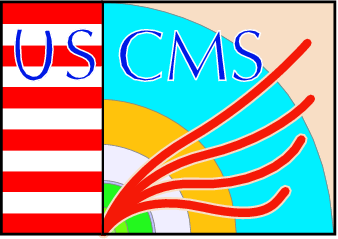
\includegraphics[height=0.6cm]{../../../Graphics/USCMS_logo.png}\hspace{.1cm}
\includegraphics[height=0.75cm]{../../../Graphics/UW_logo.png}}

\begin{document}

\begin{frame}
    \titlepage
\end{frame}

\section{Overview}
\begin{frame}
    \tableofcontents
\begin{itemize}
	\item OSG Storage Forum held at FNAL from 30 June to 01 July
	\item Agenda: \url{http://indico.fnal.gov/conferenceOtherViews.py?view=standard&confId=2538}
\end{itemize}
\end{frame}

\begin{frame}
\frametitle{Goals for the year (F. W\"urthwein)}
\begin{itemize}
	\item Support LHC users doing real work, especially at Tier3s
	\item Make life easier for storage administrators
	\begin{itemize}
		\item Simplify deployment and upgrades
		\item Improve technical support for sites
	\end{itemize}
	\item Increase Tier2 scale
	\begin{itemize}
		\item O(1M) files, 200-600 TB, 10-100 Hz to SRM via WAN, 1k-10k cores
		\item Limit maintenance cost to $<$ 0.5 FTE
	\end{itemize}
	\item Improve storage reliability at the Tier2s
	\begin{itemize}
		\item 80\% success rate in STEP09; 90\% of job failures due to LAN read errors
		\item Inadequate provisions for replication/redundancy at Tier2s
	\end{itemize}
\end{itemize}
\end{frame}

\section{Storage Technologies}

\subsection{dCache}

% site talks
% development plans
\subsection{Hadoop}
% scalability of bestman+hadoop
\subsection{Lustre}
\subsection{Xrootd}

\section{Storage in the OSG}
\subsection{Information Services}
% gip, GLUE/search tool
\subsection{Packaging}
% toolkit, VDT

\end{document}
